



\chapter{Further analysis of epistasis under selection on extended set of patterns}
\label{AppendixA}
\lhead{Appendix A. \emph{Epistasis under selection}}

\begin{figure}
\begin{center}
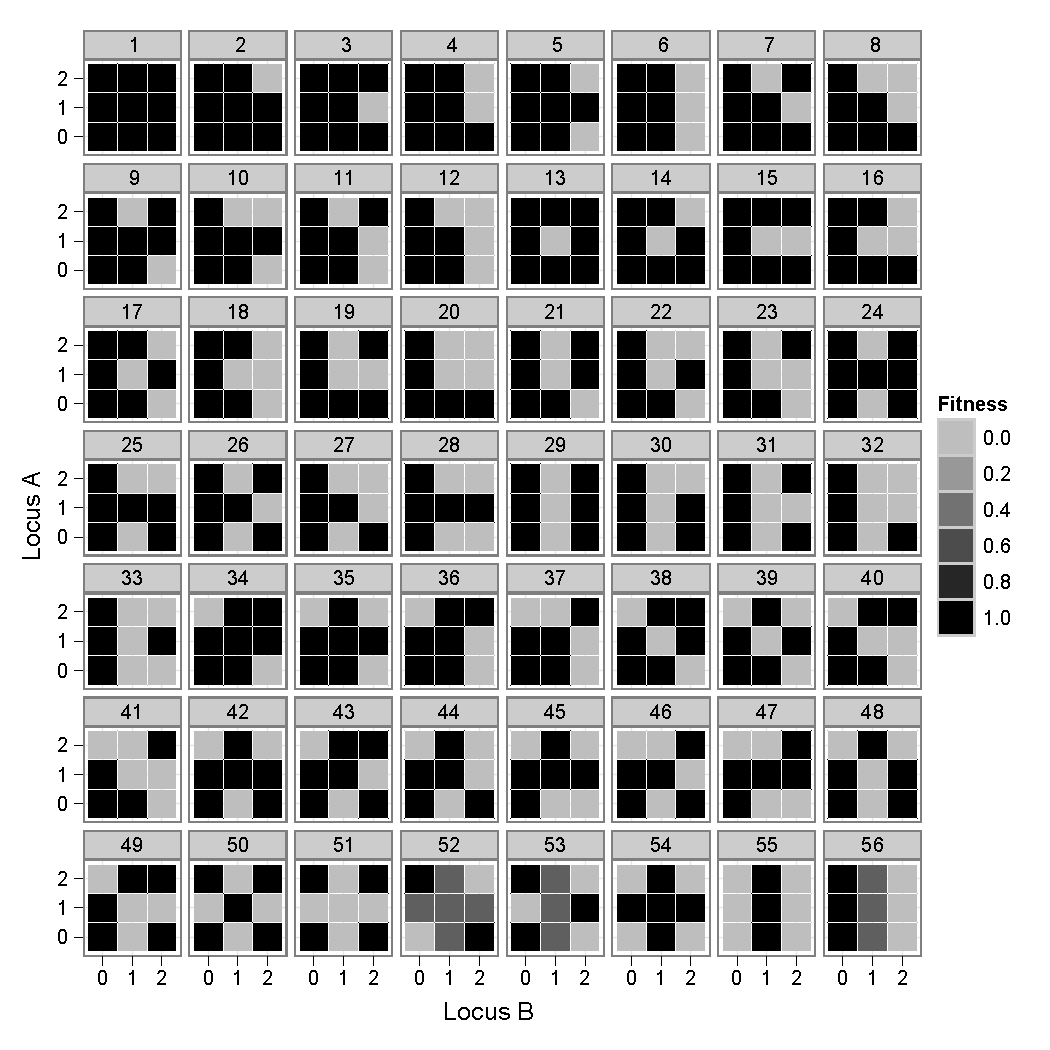
\includegraphics[scale=0.65]{Chapter1/sup_gpmaps.pdf}
\caption[Extended set of genotype-phenotype maps]{Extended set of genotype phenotype maps. \emph{1} Neutral; \emph{2-51} Enumeration of all binary trait patterns, excluding reflections, rotations and inversions, as derived by \citet{Li2000} (6 and 29 are non-episatatic); \emph{52-56} Additive x Additive, Additive x Dominance, Dominance x Dominance, Over-dominance, additive.}
\label{fig:sup_gpmaps}
\end{center}
\end{figure}

\begin{figure}
\begin{center}
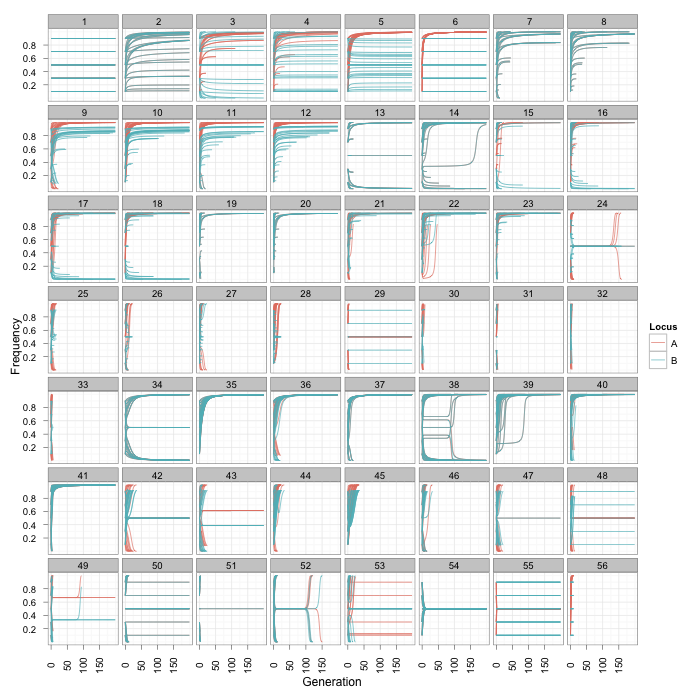
\includegraphics[scale=0.6]{Chapter1/sup_allelefreq_det.png}
\caption[Deterministic trajectory of allele frequencies for extended maps]{Deterministic trajectory of allele frequencies as in figure \ref{fig:allelefreq_det}, but for an extended set of patterns (detailed in figure \ref{fig:sup_gpmaps})}
\label{fig:sup_allelefreq_det}
\end{center}
\end{figure}

\begin{figure}
\begin{center}
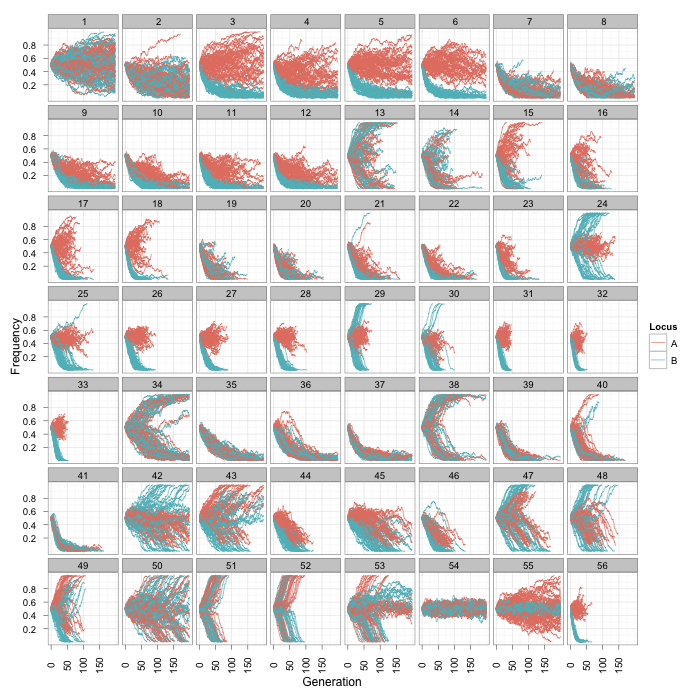
\includegraphics[scale=0.6]{Chapter1/sup_allelefreq_sim.png}
\caption[Simulated trajectory of allele frequencies for extended maps for extended maps]{Simulated trajectory of allele frequencies as in figure \ref{fig:allelefreq_sim}, but for an extended set of patterns (detailed in figure \ref{fig:sup_gpmaps})}
\label{fig:sup_allelefreq_sim}
\end{center}
\end{figure}

\begin{figure}
\begin{center}
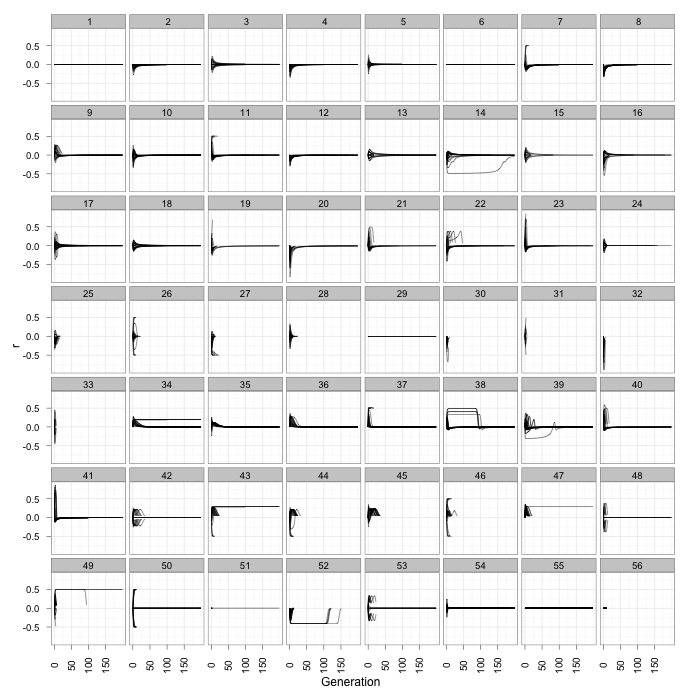
\includegraphics[scale=0.6]{Chapter1/sup_r_det.png}
\caption[Deterministic calculations of quasi-LD for extended maps]{For the 25 deterministic simulations the expected quasi-LD between the physically unlinked causal SNPs was calculated. It can be seen that significant levels are generated, such that orthogonal standard parameterisation methods would not be orthogonal. Boxes represent different genotype-phenotype maps from figure \ref{fig:sup_gpmaps}.}
\label{fig:sup_r_det}
\end{center}
\end{figure}

\begin{figure}
\begin{center}
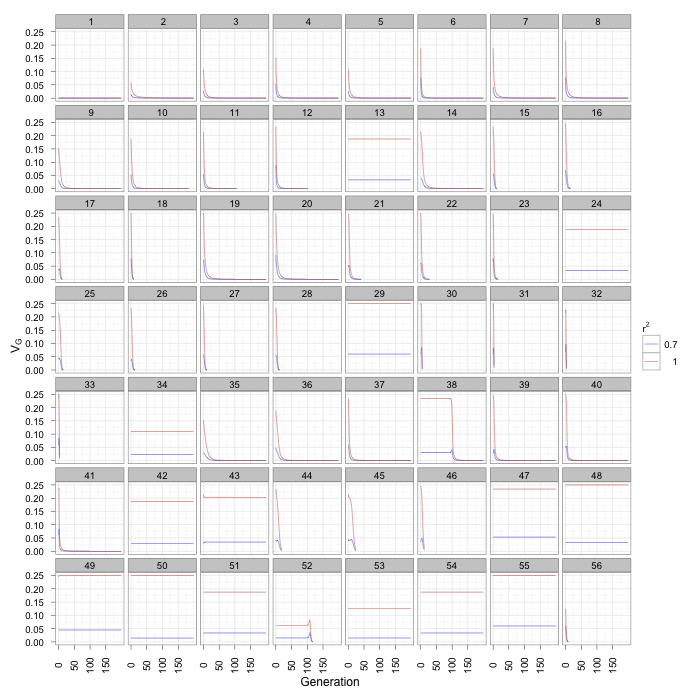
\includegraphics[scale=0.6]{Chapter1/sup_Vg_det.png} \\
\caption[Deterministically calculated change in genetic variance for extended maps]{Deterministic change in genetic variance for loci under selection exhibiting various epistatic patterns (figure \ref{fig:sup_gpmaps}), when LD between the causal variants and observed SNPs varies. For clarity, only the results from initial frequencies of 0.5 at both loci are shown. Boxes represent different genotype-phenotype maps from figure \ref{fig:sup_gpmaps}.}
\label{fig:sup_Vg_det}
\end{center}
\end{figure}

\begin{figure}
\begin{center}
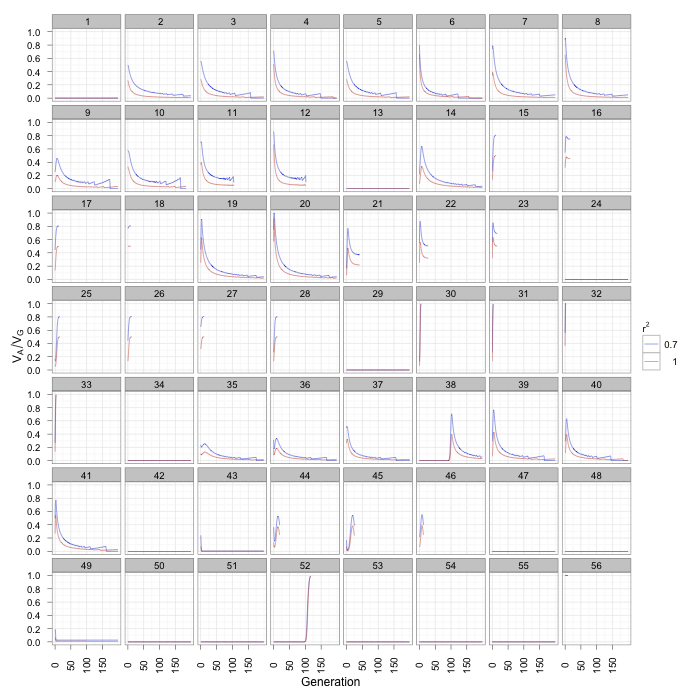
\includegraphics[scale=0.6]{Chapter1/sup_propadditive_det.png} \\
\caption[Deterministically calculated change in additive variance for extended maps]{As in figure \ref{fig:sup_Vg_det}, but this time showing the proportion of the genetic variance that is additive.}
\label{fig:sup_propadditive_det}
\end{center}
\end{figure}

\begin{figure}
\begin{center}
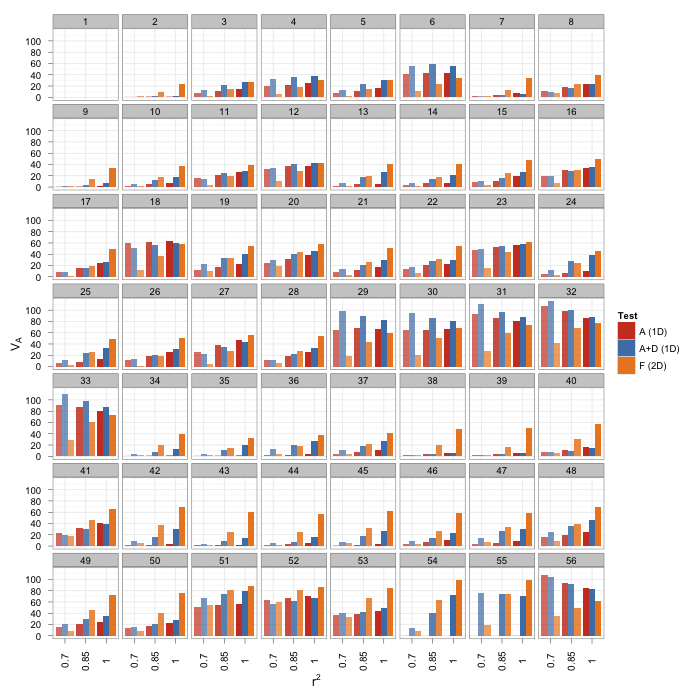
\includegraphics[scale=0.6]{Chapter1/sup_heritbars_sim.png} \\
\caption[Proportion of additive variance detected for extended maps]{As in figure \ref{fig:heritbars_det}, but for only three tests - Additive in one dimension (A (1D)), genotype in one dimension (A+D (1D)), and full epistatic in two dimensions (F (2D)). Each box has the additive variance detected across all populations and generations as a proportion of the total additive variance that was created for each test when the observed SNPs were in varying levels of LD with the causal variants. For 44 patterns the full epistatic test is most powerful when $r^{2}=1$, but when $r^{2} = 0.7$ it is never the most powerful, rather 39 patterns are best detected by the one dimensional genotype parameterisation}
\label{fig:sup_heritbars_det}
\end{center}
\end{figure}

